\section{The Chromatic Number of the Plane}

Every graph so far has been finite. The plane gives us an infinite one to colour: we will trap its chromatic number between $4$ and $7$, and then see that only its finite subgraphs matter.

\subsection{The Unit Distance Graph}

The graph in question has a vertex for every point of the plane.

\begin{boxdefinition}[Unit Distance Graph]
    The \textbf{unit distance graph} on $V = \R^2$ is given by the adjacency relation $u \sim v$ iff $\norm{u - v} = 1$.
\end{boxdefinition}

Write $G$ for this graph. What is $\chi(G)$?

One clear lower-bound on $\chi(G)$ is $3$: $G$ contains the equilateral triangle with side length $1$ as a subgraph.

It turns out that there is a subgraph of $G$ with chromatic number $4$, known as Moser's Spindle.
\begin{figure}[H]
    \centering
    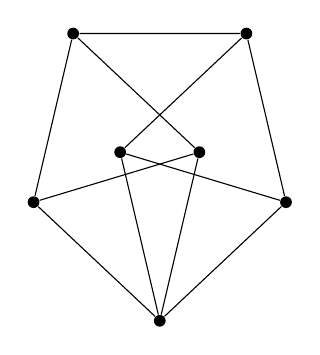
\begin{tikzpicture}[scale = 2.2]
        \node[circle, fill = black, inner sep = 1.5pt] (a) at (0, 0) {};
        \node[circle, fill = black, inner sep = 1.5pt] (p1) at (76.7787:1) {};
        \node[circle, fill = black, inner sep = 1.5pt] (q1) at (136.7787:1) {};
        \node[circle, fill = black, inner sep = 1.5pt] (t1) at (106.7787:1.7321) {};
        \node[circle, fill = black, inner sep = 1.5pt] (p2) at (43.2213:1) {};
        \node[circle, fill = black, inner sep = 1.5pt] (q2) at (103.2213:1) {};
        \node[circle, fill = black, inner sep = 1.5pt] (t2) at (73.2213:1.7321) {};
        \draw (a) -- (p1) -- (q1) -- (a);
        \draw (p1) -- (t1) -- (q1);
        \draw (a) -- (p2) -- (q2) -- (a);
        \draw (p2) -- (t2) -- (q2);
        \draw (t1) -- (t2);
    \end{tikzpicture}
\end{figure}
We thus conclude that $\chi(G) \geq 4$.

We can actually show that $\chi(G) \leq 7$. Indeed, consider the hexagonal tessellation of the plane. The point is that for a tessellation with hexagons of some diameter,
\begin{enumerate}
    \item all points in any given hexagon are of the same colour
    \item each hexagon and its $6$ neighbours have different colours
\end{enumerate}
Then, we can repeat colours \textit{after} a unit of $7$ (consisting of a hexagon and its neighbours).

% [FILLED] the diameter of the hexagons, and why the colouring is proper, supplied on 2026-10-07; the lecture gave neither
Take the hexagons to have diameter $d$ with $\frac{2}{\sqrt{21} - 2} < d < 1$---say $d = 0.9$---and give each boundary point to just one of the hexagons it lies on. Two points of one hexagon are less than $1$ apart, so giving a hexagon a single colour breaks nothing. The centres of neighbouring hexagons are $\frac{\sqrt{3}}{2} d$ apart, and in the colouring below the nearest hexagon of the same colour as a given one is two steps away in one direction and one in the next, so two same-coloured centres are at distance at least $\sqrt{7} \cdot \frac{\sqrt{3}}{2} d = \frac{\sqrt{21}}{2} d$. Every point of a hexagon is within $\frac{d}{2}$ of its centre, so two points of the same colour in different hexagons are at distance at least $\frac{\sqrt{21}}{2} d - d > 1$. No two points at distance exactly $1$ share a colour, and $\chi(G) \leq 7$.
\begin{figure}[H]
    \centering
    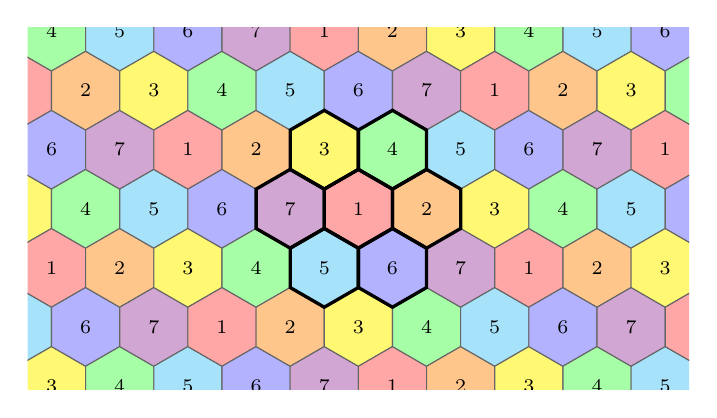
\begin{tikzpicture}
        \def\hexfills{{"red!35", "orange!45", "yellow!55", "green!35", "cyan!35", "blue!30", "violet!35"}}
        \clip (-4.2, -2.3) rectangle (4.2, 2.3);
        \foreach \hq in {-8, ..., 8}{
            \foreach \hr in {-4, ..., 4}{
                \pgfmathsetmacro{\x}{0.866 * (\hq + 0.5 * \hr)}
                \pgfmathsetmacro{\y}{0.75 * \hr}
                \pgfmathtruncatemacro{\hexc}{mod(mod(\hq + 3 * \hr, 7) + 7, 7)}
                \pgfmathtruncatemacro{\hexnum}{\hexc + 1}
                \pgfmathparse{\hexfills[\hexc]}
                \edef\hexfill{\pgfmathresult}
                \filldraw[fill = \hexfill, draw = black!60, shift = {(\x, \y)}] (30:0.5) -- (90:0.5) -- (150:0.5) -- (210:0.5) -- (270:0.5) -- (330:0.5) -- cycle;
                \node[font = \scriptsize] at (\x, \y) {$\hexnum$};
            }
        }
        \foreach \hq/\hr in {0/0, 1/0, -1/0, 0/1, 0/-1, 1/-1, -1/1}{
            \pgfmathsetmacro{\x}{0.866 * (\hq + 0.5 * \hr)}
            \pgfmathsetmacro{\y}{0.75 * \hr}
            \draw[very thick, shift = {(\x, \y)}] (30:0.5) -- (90:0.5) -- (150:0.5) -- (210:0.5) -- (270:0.5) -- (330:0.5) -- cycle;
        }
    \end{tikzpicture}
\end{figure}

\subsection{Compactness}

Now for a topological detour!

Recall that a space is compact iff the closed sets satisfy the finite intersection property: for closed sets $Y_{\alpha}$, with $\alpha \in I$, if $\bigcap_{\alpha \in J} Y_{\alpha}$ is nonempty for all finite $J \ssq I$, then $\bigcap_{\alpha \in I} Y_{\alpha}$ is nonempty as well.

We'll use this property (and Tychonoff) to prove a `compactness theorem' for the chromatic number of the plane.

\begin{boxtheorem} \label{Ch2:Thm:Compactness_Chromatic}
    For any graph $G$,
    \begin{align*}
        \chi(G) = \sup\setst{\chi(H)}{H \ssq G \text{ and } H \text{ is finite}}
    \end{align*}
\end{boxtheorem}

First, a lemma.

\begin{boxlemma} \label{Ch2:Lemma:Compactness}
    If every finite subgraph $B$ of $G$ is $k$-colourable, then so is $G$.
\end{boxlemma}
\begin{proof}
    Consider $[k]$ with the discrete topology and $[k]^{V(G)}$ with the product topology. Note that $[k]^{V(G)}$ is the set of all (not necessarily proper) colourings of $G$.

    For all $e \in E(G)$, define
    \begin{align*}
        P_e = \setst{c \in [k]^{V(G)}}{c(u) \ne c(v) \text{ for } e = \set{u, v}}
    \end{align*}
    It is possible to show that $P_e$ is clopen in $[k]^{V(G)}$: it is the preimage of the clopen set $\setst{(a, b) \in [k]^2}{a \neq b}$ under the projection onto the coordinates $u$ and $v$, which is continuous. % [FILLED] the reason after the colon was supplied on 2026-10-07

    % [FILLED] from ``the edges in $J$'' to the end of the proof, supplied on 2026-10-07: the lecture stopped at the display
    If every finite subgraph can be $k$-coloured, then for all finite $J \ssq E(G)$, $\bigcap_{e \in J} P_{e} \ne \emptyset$: the edges in $J$ span a finite subgraph, a proper $k$-colouring of it extends to all of $V(G)$ by colouring the remaining vertices arbitrarily, and the result lies in every $P_e$ with $e \in J$. By Tychonoff's theorem $[k]^{V(G)}$ is compact, the $P_e$ are closed, and so the finite intersection property gives $\bigcap_{e \in E(G)} P_e \ne \emptyset$. Any $c$ in that intersection has $c(u) \ne c(v)$ for every edge $\set{u, v}$, ie, is a proper $k$-colouring of $G$.
\end{proof}

% [FILLED] the deduction of the theorem from the lemma, supplied on 2026-10-07; the lecture stated the theorem, said ``first, a lemma'', and never came back
\begin{proof}[Proof of \Cref{Ch2:Thm:Compactness_Chromatic}]
    Every subgraph $H$ of $G$ has $\chi(H) \leq \chi(G)$, so the supremum is at most $\chi(G)$. Conversely, if the supremum is some finite $k$, then every finite subgraph is $k$-colourable, so $G$ is by \Cref{Ch2:Lemma:Compactness}, and $\chi(G) \leq k$.
\end{proof}
